\documentclass[10pt,a4paper]{report}
\usepackage[left=3.00cm, right=1.00cm, top=2.00cm, bottom=2.00cm, nohead, footskip=7mm]{geometry}
\usepackage[14pt]{extsizes}

\usepackage[utf8]{inputenc}
\usepackage[T1]{fontenc}
\usepackage{amsmath}
\usepackage{amsfonts}
\usepackage{amssymb}
\usepackage{pdfpages}

\usepackage[russian]{babel}

% Ссылки внутри текста
\usepackage{hyperref}

% Отступ абзаца
\usepackage{indentfirst}
\setlength{\parindent}{1.5cm} 

% Межстрочный интервал
\usepackage{setspace}
\onehalfspacing % интервал 1.5

% Вставка изображений
\usepackage{graphicx}
\graphicspath{{../schemes/}}

% Настройка оглавлений
\usepackage{titlesec}
\newcommand{\hsp}{\hspace{20pt}}
\titleformat{\chapter}[hang]{\large\bfseries}{\thechapter{. }}{0pt}{\large\bfseries}
\titlelabel{hlabel-formati}
\titlespacing{\chapter}{42pt}{-80pt}{12pt}
\titleformat{\section}[hang]{\large\bfseries}{\thesection{. }}{0pt}{\large\bfseries}
\titlespacing{\section}{42pt}{12pt}{5pt plus 5pt}

% Настройка списков
\usepackage{enumitem}
\setlist{nolistsep, itemsep=0.3cm,parsep=0pt,leftmargin=1.9cm}

% Настройка листингов
\usepackage{listings}
\lstset{
	language = c++,
	extendedchars=\true,
	keepspaces=true,
	basicstyle=\small\sffamily,
	showstringspaces=\false,
	numbers=left,
	stepnumber=1,
	numbersep=5pt,
	frame=single,
	tabsize=2,
	captionpos=t,
	breaklines=true,
	breakatwhitespace=false,
	escapeinside={\#*}{*)}
}



\begin{document}
	\renewcommand\bibname{Список литературы}
	
	\includepdf[pages=1]{title.pdf}
	
	\tableofcontents
	\newpage

	\chapter*{Введение}
	\addcontentsline{toc}{chapter}{Введение}
	Трудоёмкость алгоритма - это зависимость стоимости операций от линейного размера входа\cite{perf_def}.

Модель вычислений трудоёмкости имеет следующие оценки:
\begin{itemize}
	\item Оценка стоимости базовых операций. Операции =, +, - и т.д. имеют стоиость 1.
	\item Оценка циклов. Включает в себя стоимость тела цикла, сравнения и инкремента.
	\item Оценка условного оператора if. Производится оценка обоих случаев.
\end{itemize}

Оценка характера трудоёмкости даётся по наиболее быстрорастущему слагаемому. Такая оценка играет важную роль в 
разработке и анализе алгоритмов, так как позволяет судить об оптимальности использования алгритма при тех или
иных входных данных.

В данной лабораторной оценивается трудоёмкость классического алгоритма умножения матриц и алгоритма Винограда. 

	\newpage

	\chapter{Аналитическая часть}
	Целью лабораторной работы является оценка трудоёмкости алгоритмов сортировки.

Выделены следующие задачи лабораторной работы:

\begin{itemize}
\item описание операции сортировки;
\item описание и реализация алгоритмов сортировки;
\item проведение замеров процессорного времени работы алгоритмов при различных размерах массивов;
\item оценка трудоёмкости алгоритов;
\item проведение сравнительного анализа алгоритмов на основании экспериментов.
\end{itemize}

Сортировка массива по неубыванию - операция над массивом $arr[N]$, в результате которой в нём начинает выполняется условие:
\begin{equation} 
	arr[i+1] >= arr[i], i \in [0, N-2]
\end{equation}

Аналогично формулируется определение для сортировки по невозрастанию. В случае, если в массиве нет равных элементов, также возможно применить операции сортироки по возрастанию и убыванию.

	\newpage
	
	\chapter{Конструкторская часть}
	Рассмотрим вышеупомянутые алгоритмы сортировки. Для удобства изложения сути алгоритмов, будем рассматривать сортировку по неубыванию. Алгоритмы сортировки других порядков могут быть получены заменой условия сравнения.

\section{Сортировка пузырьком}
Алгоритм сортировки пузырьком основывается на следующем действии. Массив проссматривается от 0 до N-2 элемента, и в случае, если текущий элемент массива больше следующего, они меняются местами. Таким образом, после первого прохода в конце массива окажется максимальный элемент, после второго - два максимальных, и так далее до полного упорядочивания массива.

Схема алгоритма приведена на рисунке 2.1.
\begin{figure}[h]
	\begin{center}
		{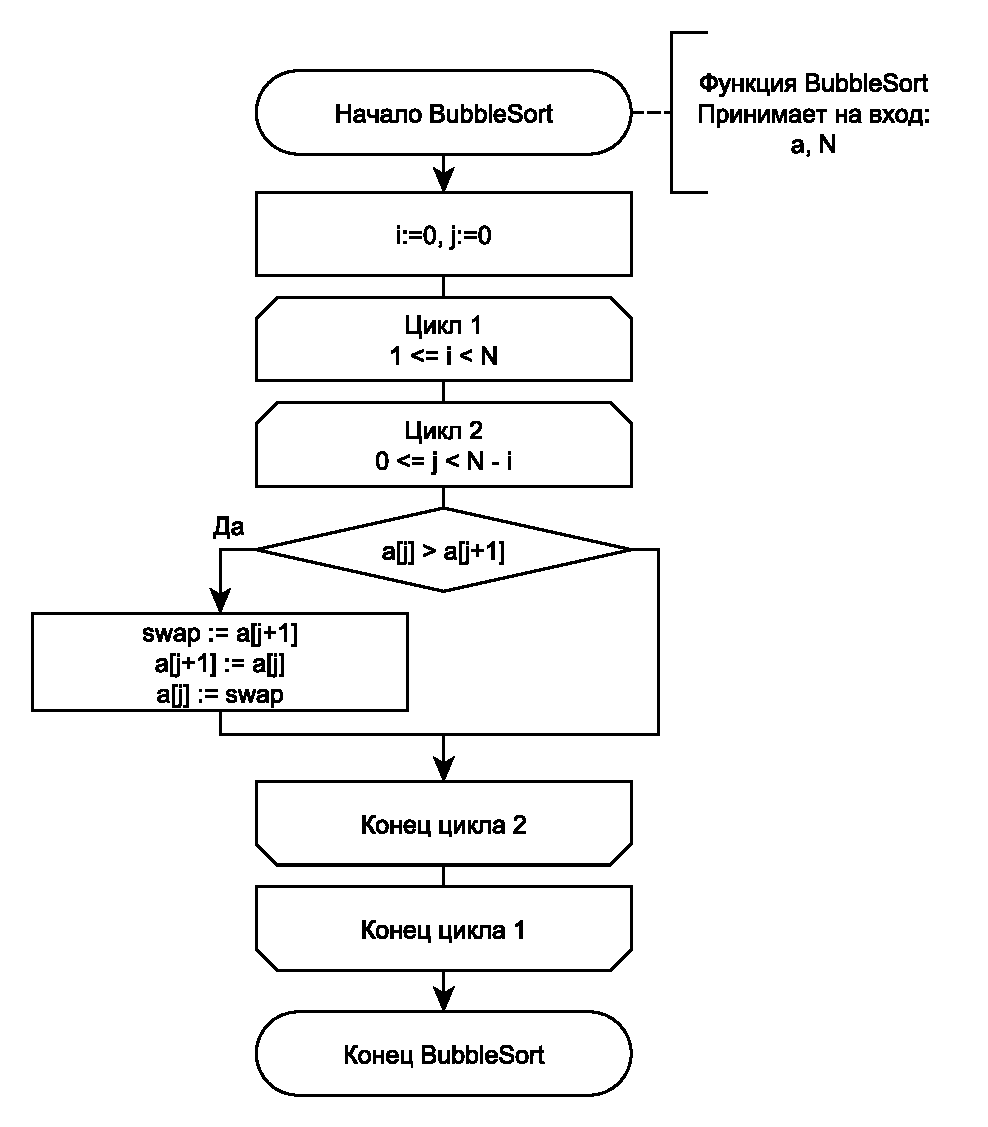
\includegraphics[height=20cm, width = 17cm]{Bubble}}
		\caption{Сортировка пузырьком}
	\end{center}
\end{figure}


\section{Поразрядная сортировка}
Цель алгоритма заключается в реализации трудоёмкости, линейно зависящей от размера массива. Упорядоченнсть достигается последовательной сортировкой по значению разрядов (в порядке от меньшего разряда к большему). Алгоритм применим к массиву, состоящему из целых положительных чисел или иных значений, которые м.б. спроецированы на множетво положительных чисел \cite{Korman}. 

Будем считать, что максимальное число в массиве состоит из K разрядов. В случае, если массив содержит целыйе отрицательные числа, то перед сортировкой все числа должны быть увеличены на модуль минимального числа, а после сортировки уменьшены.

Схема алгоритма приведена на рисунках 2.2. и 2.3.
\begin{figure}[h]
	\begin{center}
		{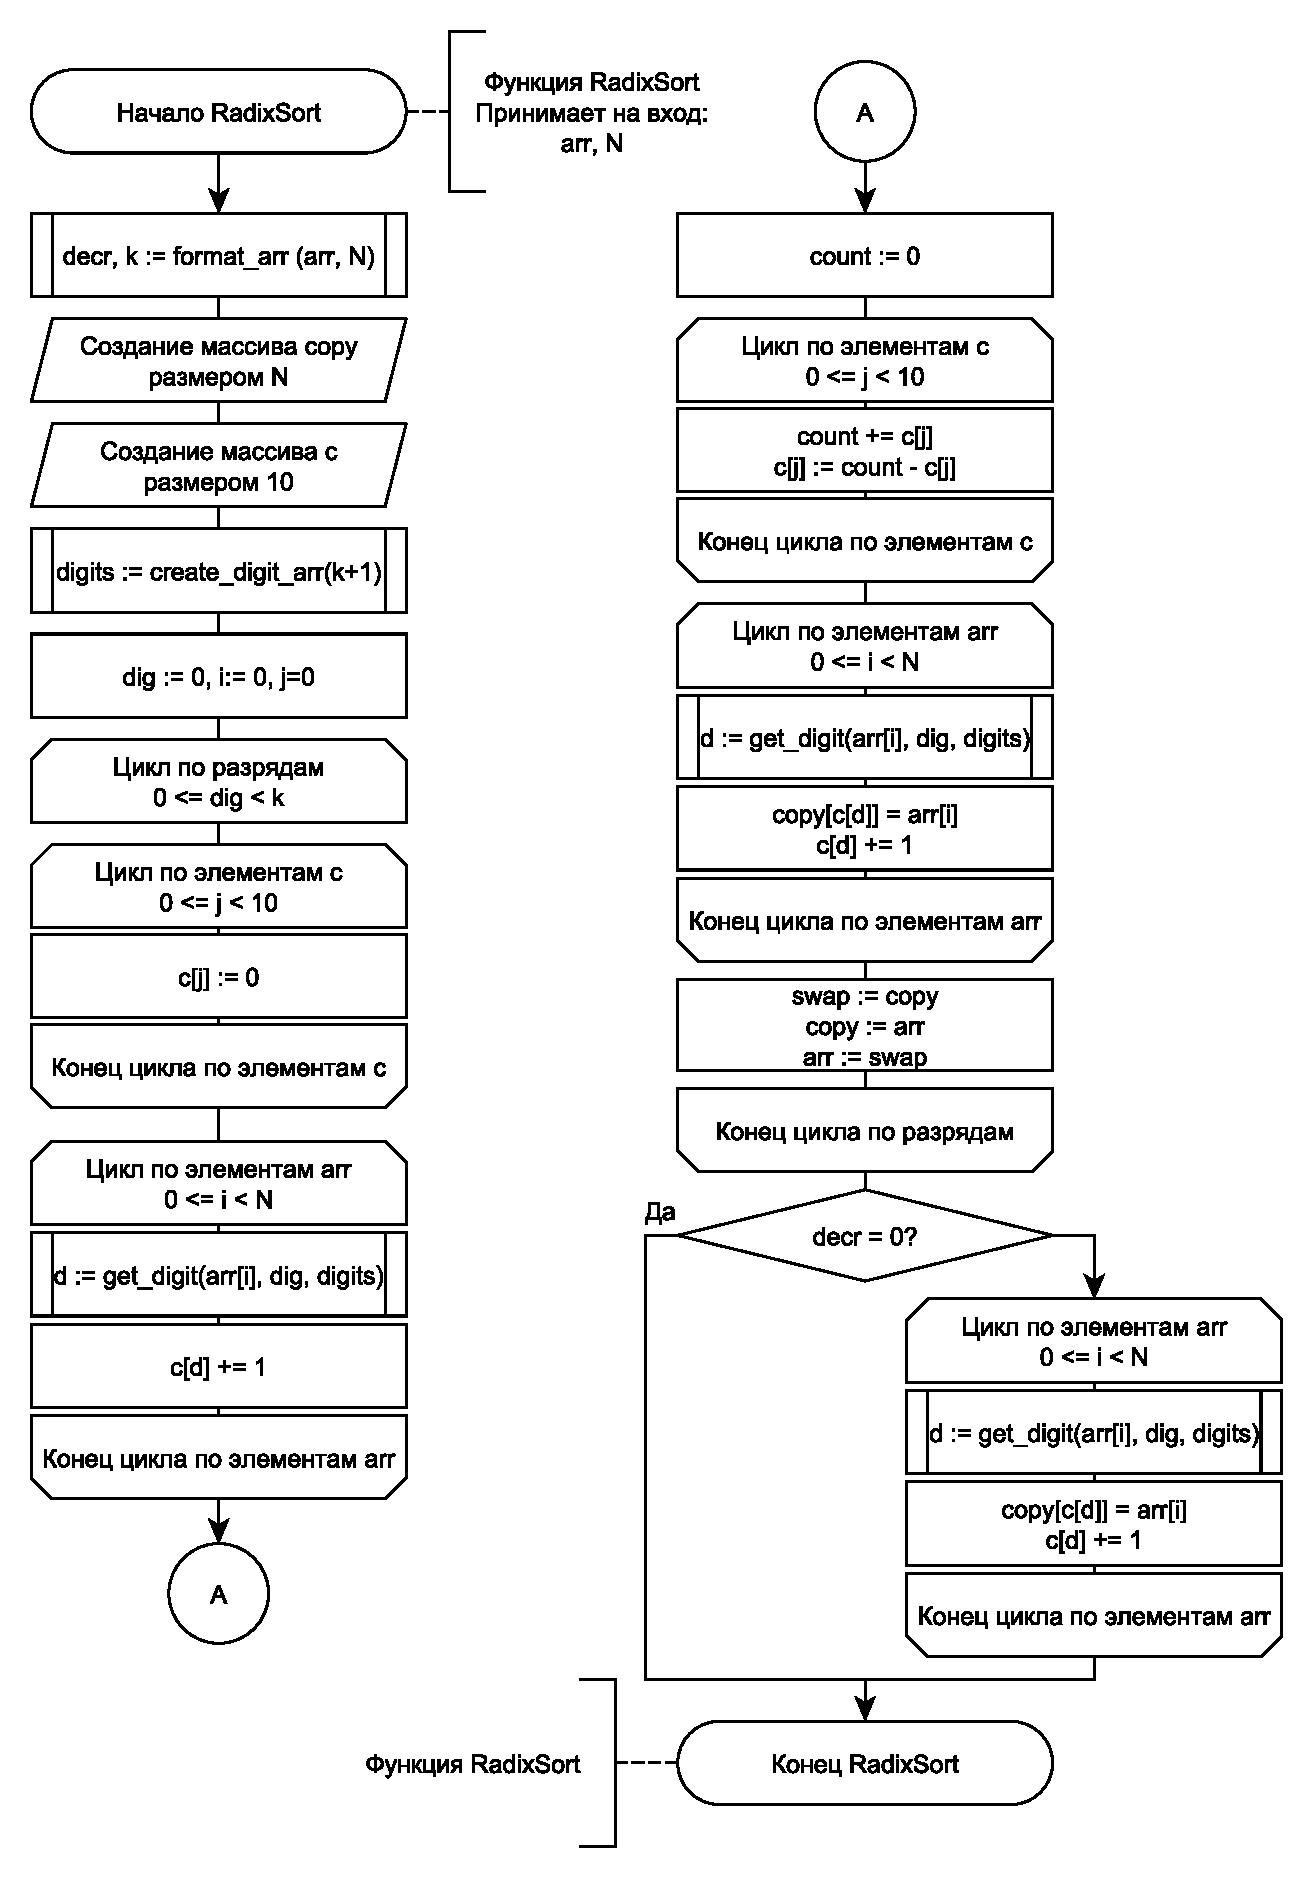
\includegraphics[height=20cm]{Radix1}}
		\caption{Поразрядная сортировка (часть 1)}
	\end{center}
\end{figure}

\begin{figure}[h]
	\begin{center}
		{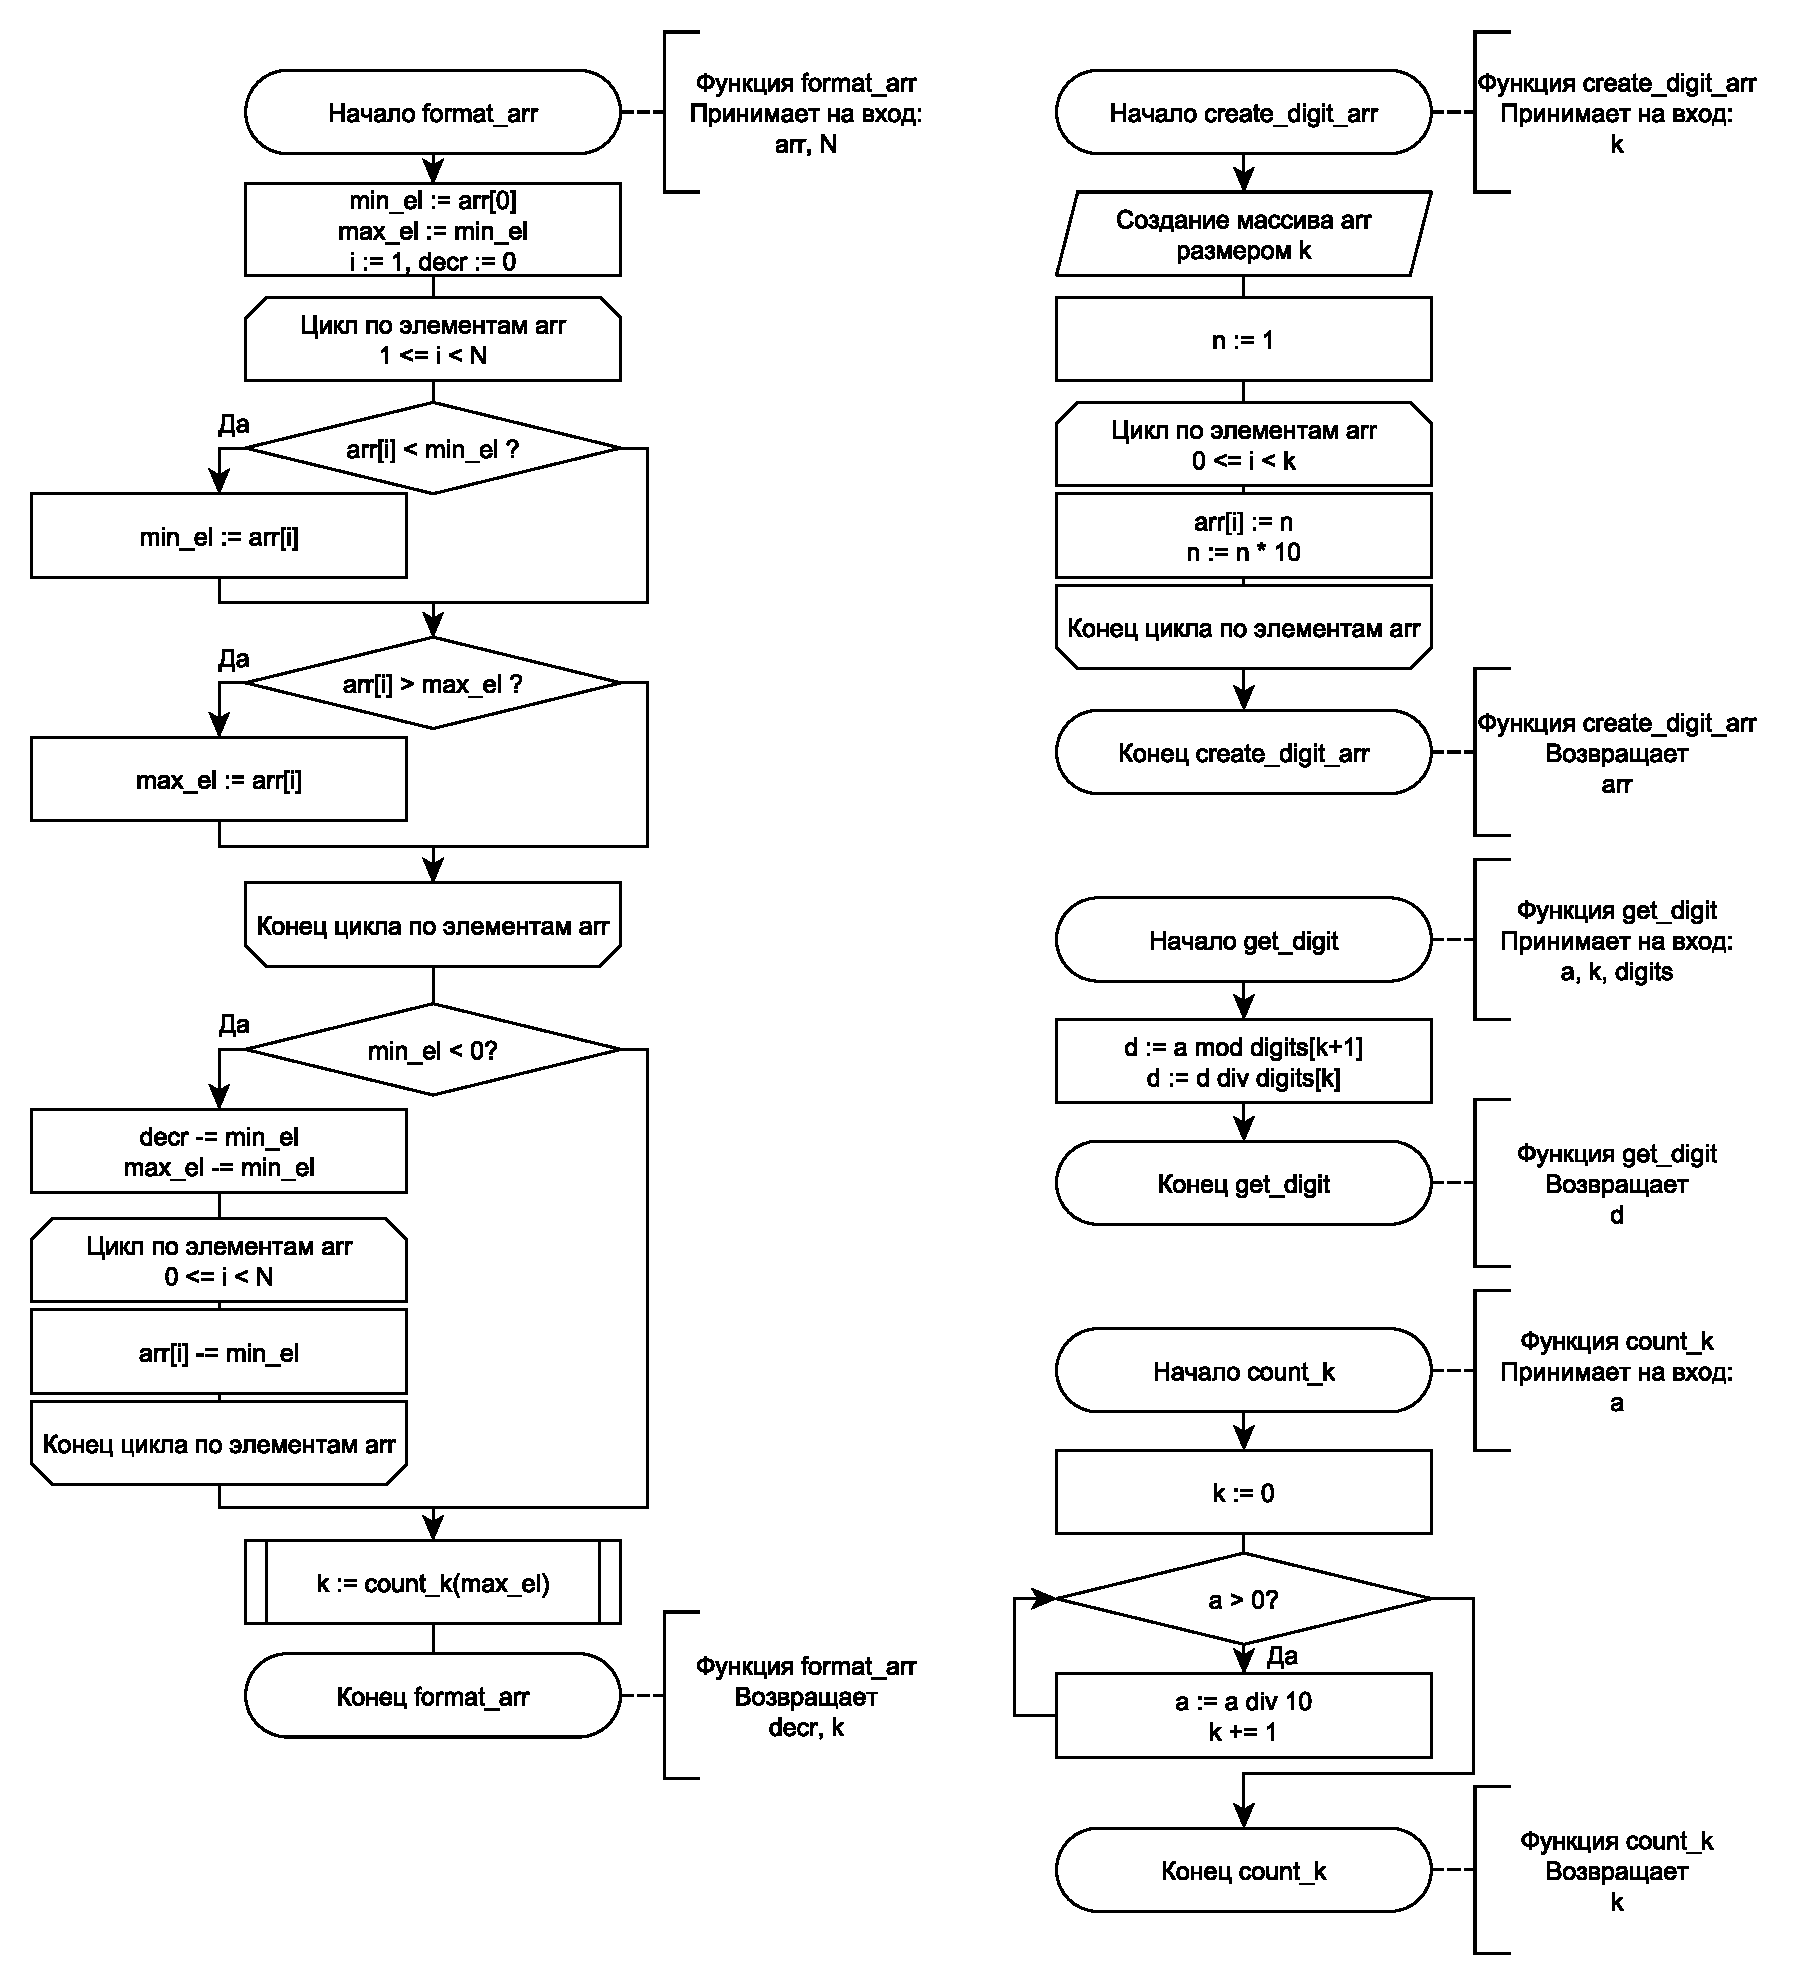
\includegraphics[width = 17cm]{Radix2}}
		\caption{Поразрядная сортировка (часть 2)}
	\end{center}
\end{figure}


\section{Сортировка слиянием}
Идея алгоритма заключается в том, что достаточно эффективно производится операция слияния (т.е. создания из двух массивов одного) при условии, что оба сливаемых массива уже упорядочены. Алгоритм разбивает массив на два подмассива, после чего применяет к ним ту же операцию, до тех пор, пока длина массива не станет меньше 3. После завершения сортировки подмассивов производится построение упорядоченного массива их слиянием.

Схема алгоритма приведена на рисунке 2.4.
\begin{figure}[h]
	\begin{center}
		{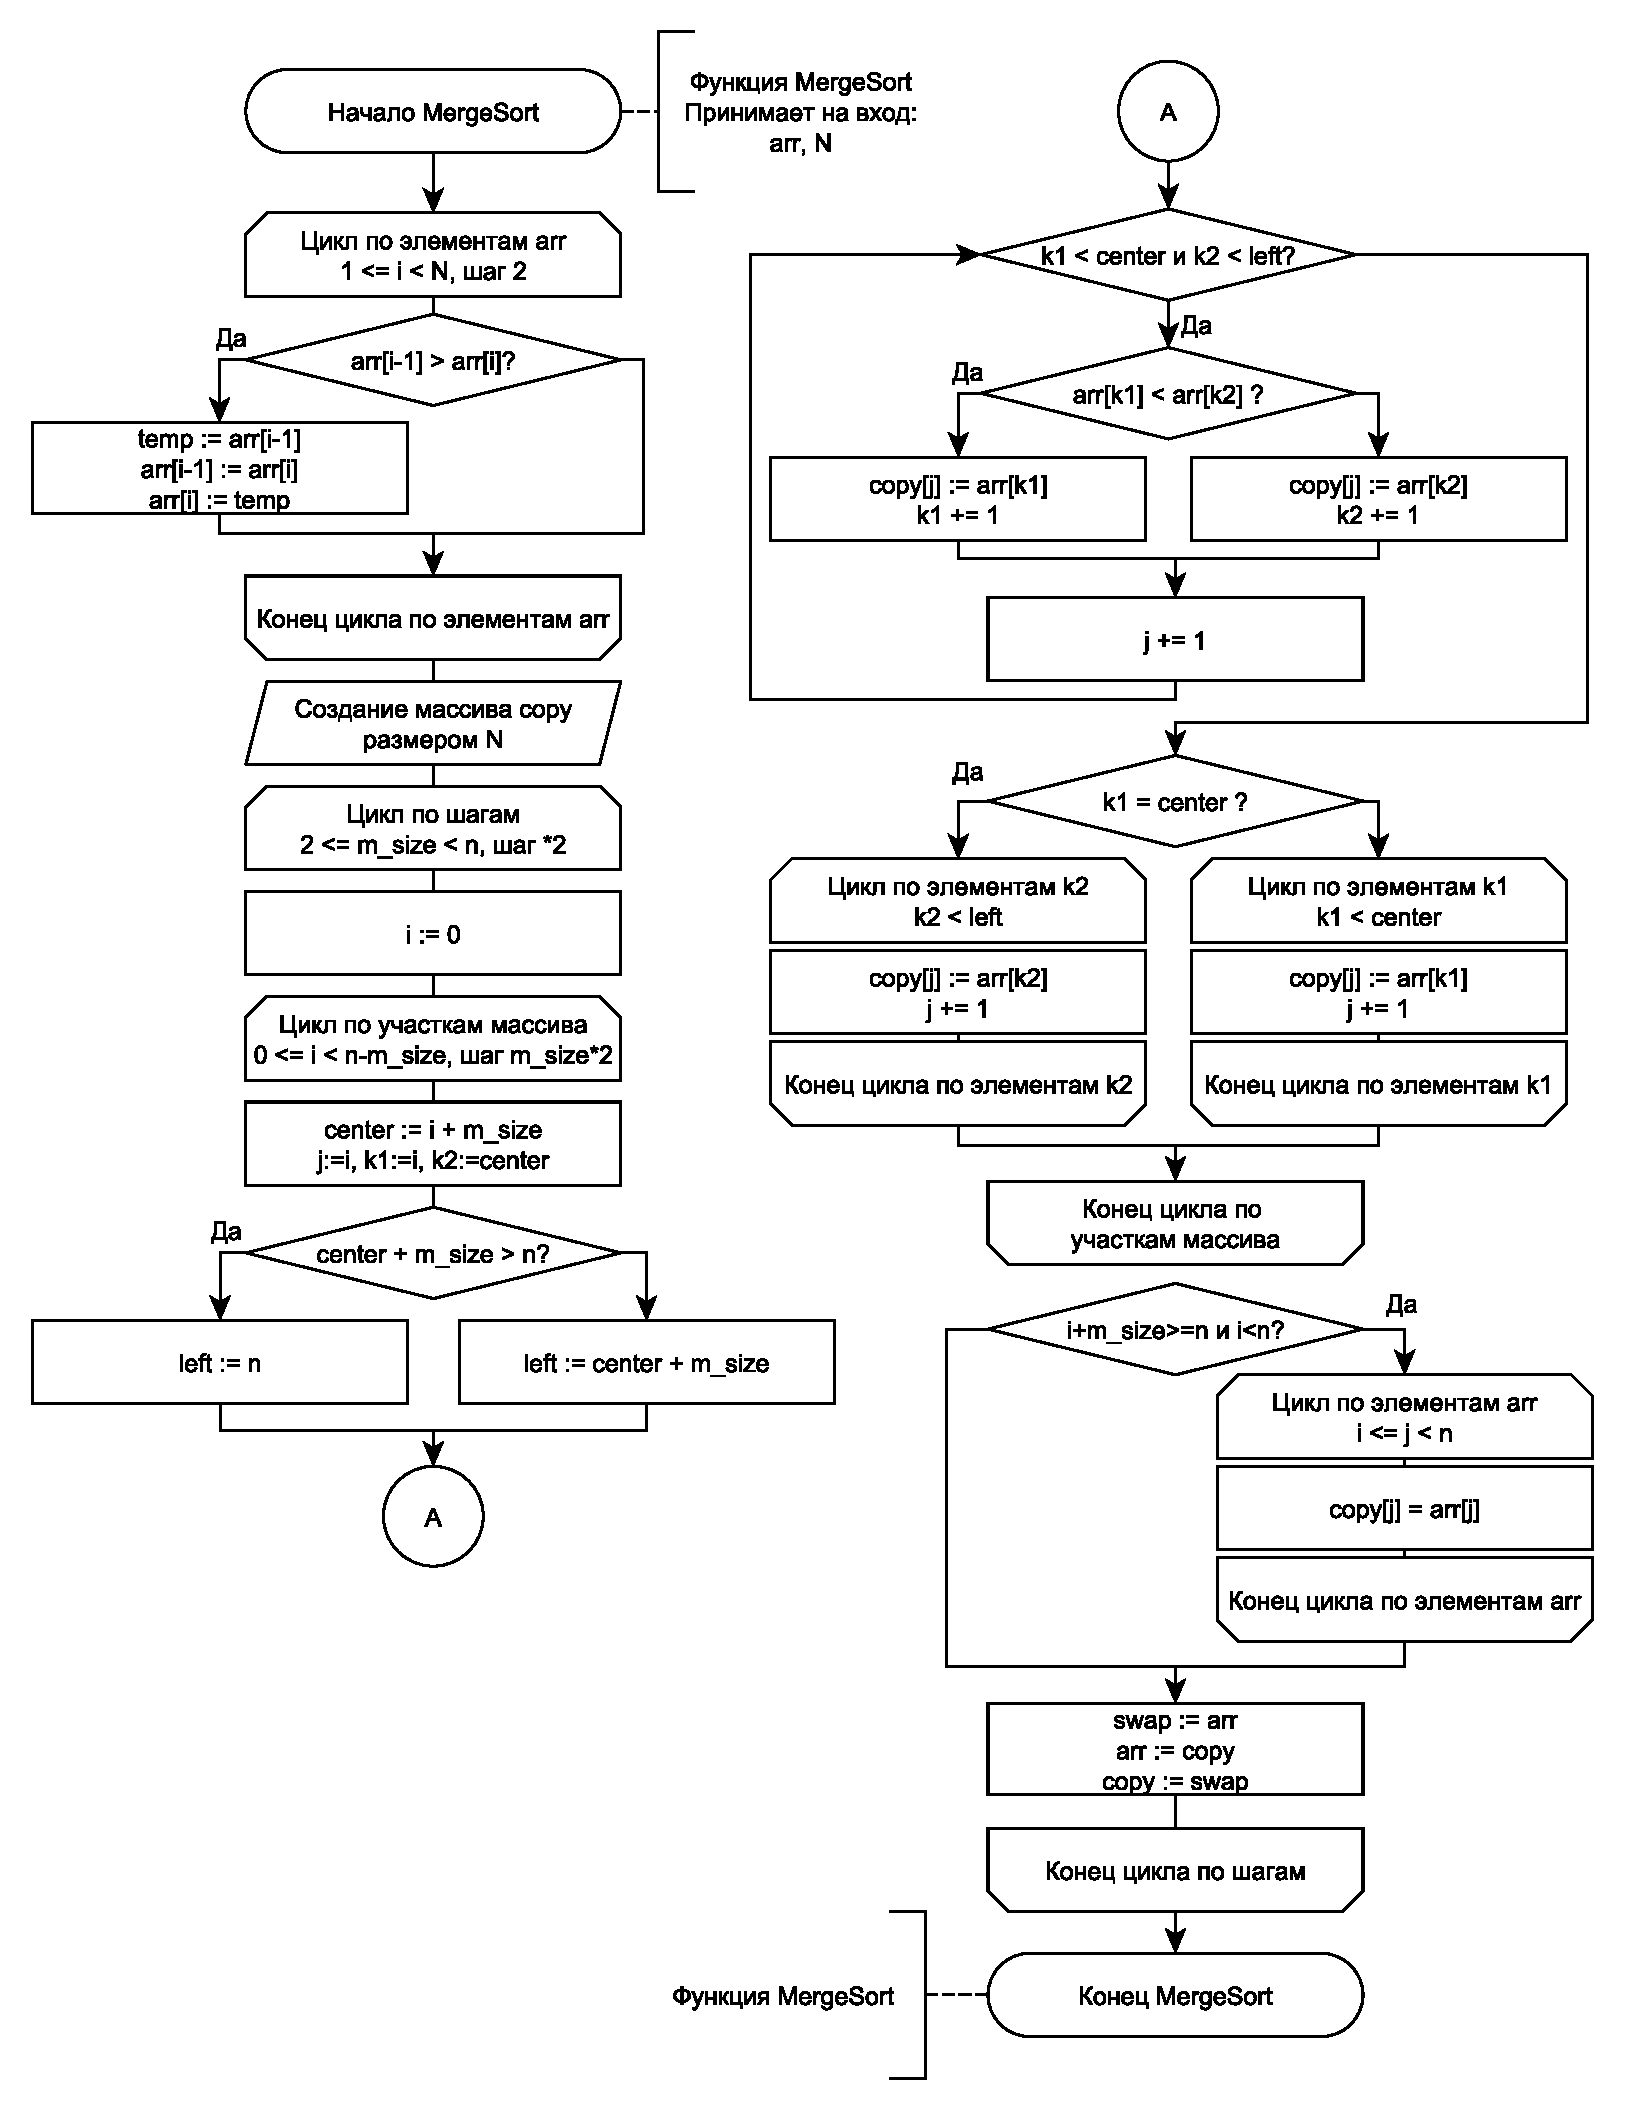
\includegraphics[height=20cm]{Merge}}
		\caption{Сортировка слиянием}
	\end{center}
\end{figure}


\section{Требования к программному обеспечению}
Для полноценной проверки и оценки алгоритмов необходимо выполнить следующее.
\begin{enumerate}
	\item Обеспечить возможность консольного ввода массива и выбора алгоритма сортировки. Программа должна вывести отсортированный массив.
	\item Реализовать функцию замера процессорного времени, затраченного функцией. Для этого также создать возможность ввода размера массива, на котором будет выполнен замер.
\end{enumerate}


\section{Заготовки тестов}
При проверке алгоритмов необходимо будет использовать следующие классы тестов:
\begin{itemize}
	\item массив размером 1;
	\item массив одинаковых элементов;
	\item упорядоченный и обратно упорядоченный массив.
\end{itemize}

\section*{Вывод}
Результатом конструкторской части стало схематическое описание алгоритмов сортировок, задание требований к программному обеспечению и к системе тестов.


	\newpage

	\chapter{Технологическая  часть}
	\section{Выбор языка программирования}
В качестве языка программирования был выбран C++\cite{C++_Doc}, так как имеется опыт работы с ним, и с библиотеками, позволяющими провести исследование и тестирование программы. Разработка проводилась в среде Visual Studio 2019\cite{VisualStudio}.

\section{Листинги кода}
Реализация алгоритмов поиска представлена на листингах 3.1-3.3.

\begin{lstlisting}[caption = {Поиск полным перебором}]
path_t explore_brunch(const len_matrix& m, const path_t& available_nodes, size_t cur_node, len_t& len)
{
	path_t res_path;
	len = -1;
	
	if (!available_nodes.size())
	{
		if (m[cur_node][0] < 0)
			return res_path;
		
		len = m[cur_node][0];
		res_path.push_back(0);
	}
	else
	{
		for (size_t i = 0; i < available_nodes.size(); i++)
		{
			size_t next_node = available_nodes[i];
			if (m[cur_node][next_node] < 0)
				continue;
			
			len_t temp_len = -1;
			path_t temp_nodes = available_nodes;
			temp_nodes.erase(temp_nodes.begin() + i);
			
			path_t temp_path = explore_brunch(m, temp_nodes, next_node, temp_len);
			if (temp_len < 0)
				continue;
			temp_len += m[cur_node][next_node];
			
			if (len < 0 || len > temp_len)
			{
				res_path = temp_path;
				len = temp_len;
			}
		}
	}
	
	res_path.push_back(cur_node);
	return res_path;
}

path_t brute_force(const len_matrix& m, len_t& len)
{
	path_t full_p(all_nodes(m));
	full_p.erase(full_p.begin()); // delete 0 node
	len = -1;
	path_t ans(explore_brunch(m, full_p, 0, len));
	if (ans.size() == m.size() + 1)
		return ans;
	else
	{
		len = 0;
		return path_t();
	}
}
\end{lstlisting}

\begin{lstlisting}[caption = {Поиск муравьиным алгоритмом (главная функция)}]
path_t ant_search(const len_matrix& m, ant_config& cnf)
{
	double init_tau = 1;
	double min_tau = init_tau/10;
	vector<vector<double>> tau = create_matrix(m.size(), init_tau);
	
	path_t min_path;
	len_t min_len = -1;
	size_t elite_n = 4;
	
	for (size_t t = 0; t < cnf.max_t; t++)
	{	
		ant_arr colony = init_colony(m);
		vector<vector<double>> d_tau = create_matrix(m.size(), 0);
		
		for (size_t i = 0; i < colony.size(); i++)
		{
			ant_t& ant = colony[i];
			size_t init_pos = ant.pos;
			
			while (ant.avl_nodes.size())
				if (!next_step(ant, m, tau, cnf)) 
					break;
			
			if (ant.avl_nodes.size())
			{ 
				ant.temp_len = -1;
			}
			else
			{
				ant.avl_nodes.push_back(init_pos);
				if (!next_step(ant, m, tau, cnf)) 
					ant.temp_len = -1;
			}
		}
		
		for (ant_t ant : colony)
		{
			if (ant.temp_len < 0)
				continue;

			if (min_len > ant.temp_len || min_len < 0)
			{
				min_len = ant.temp_len;
				min_path = ant.path;
			}
			
			double inc = ((double)cnf.q) / ant.temp_len;
			for (size_t i = 1; i < ant.path.size(); i++)
			{
				d_tau[ant.path[i]][ant.path[i-1]] += inc;
				d_tau[ant.path[i-1]][ant.path[i]] += inc;
			}
		}
		
		double inc = ((double)cnf.q) / min_len * elite_n;
		for (size_t i = 1; i < min_path.size(); i++)
		{
			d_tau[min_path[i]][min_path[i - 1]] += inc;
			d_tau[min_path[i - 1]][min_path[i]] += inc;
		}
		
		for (size_t i = 0; i < tau.size(); i++)
			for (size_t j = 0; j < tau.size(); j++)
				tau[i][j] = max(tau[i][j]*(1 - cnf.ro) + d_tau[i][j], min_tau);
	}
	
	return min_path;
}
\end{lstlisting}

\begin{lstlisting}[caption = {Поиск муравьиным алгоритмом (дополнительные функции)}]
ant_arr init_colony(const len_matrix& m)
{
	size_t len = m.size();
	path_t pos = all_nodes(m);
	random_shuffle(pos.begin(), pos.end());
	
	ant_arr arr(len);
	for (size_t i = 0; i < len; i++)
	{
		arr[i].pos = pos[i];
		arr[i].temp_len = 0;
		arr[i].path.push_back(pos[i]);
		
		arr[i].avl_nodes = all_nodes(m);
		arr[i].avl_nodes.erase(arr[i].avl_nodes.begin() + pos[i]);
	}
	
	return arr;
}

int get_next_node(const ant_t& ant, const len_matrix& m, const vector<vector<double>>& tau, const ant_config& cnf)
{
	size_t cur = ant.pos;
	vector<double> node_p(ant.avl_nodes.size(), 0);
	double sum_p = 0;
	
	for (size_t j = 0; j < ant.avl_nodes.size(); j++)
	{
		size_t next = ant.avl_nodes[j];
		if (m[cur][next] < 0)
			continue;
		
		double val = pow(tau[cur][next], cnf.a) / pow(m[cur][next], cnf.b);
		sum_p += val;
		node_p[j] = sum_p;
	}
	if (sum_p < 1e-9) 
		return -1; 
	
	double rand_f = ((double)rand() / RAND_MAX) * sum_p * (1 - 1e-8);
	
	for (size_t next = 0; next < node_p.size(); next++)
		if (node_p[next] > rand_f)
			return ant.avl_nodes[next];
	return ant.avl_nodes[node_p.size() - 1];
}
int next_step(ant_t& ant, const len_matrix& m, const vector<vector<double>>& tau, const ant_config& cnf)
{
	size_t cur = ant.pos;
	int next = get_next_node(ant, m, tau, cnf);
	if (next == -1)	return 0;
	
	ant.pos = next;
	ant.temp_len += m[cur][next];
	ant.path.push_back(next);
	ant.avl_nodes.erase(find(ant.avl_nodes.begin(), ant.avl_nodes.end(), next));	
	
	return 1;
}
\end{lstlisting}

\section{Автоматическая параметризация муравьиного алгоритма}
Для исследования работы муравьиного алгоритма на разных наборах функций была написана функция автоматической параметризации, приведённая в листинге 3.4.

\begin{lstlisting}[caption = {Функции автоматической параметризации муравьиного алгоритма}]
void best_config(const len_matrix& m, len_t q, len_t perfect_len)
{
	len_t min_len = q * 1000;
	ant_config best_cnf;
	for (double a = 0; a <= 1; a+=0.1)
	{
		double b = 1 - a;
		for (double ro = 0; ro <= 1; ro += 0.1)
		{
			ant_config cnf = create_config(a, ro, 30, q);
			len_t local_min = q * 1000;
			for (int i=0; i<3; i++)
			{
				path_t p = ant_search(m, cnf);
				len_t len = path_len(m, p);
				local_min = min(len, local_min);
			}
			printf("%.1lf %.1lf %.1lf %zd: %.2lf %.2lf\n", a, b, ro, cnf.max_t,	local_min, local_min - perfect_len);
			if (min_len > local_min)
			{
				min_len = local_min;
				best_cnf = cnf;
			}
		}
		printf("\n");
	}
	
	printf("%.1lf %.1lf %.1lf : %.2lf\n", best_cnf.a, best_cnf.b, best_cnf.ro, min_len);
}
\end{lstlisting}

\section{Результаты тестирования}
Для тестирования написанных функций был создан отдельный файл с ранее описанными классами тестов. Тестирование функций проводилось за счёт сравнения результов функций c ожидаемым результатом. Отдельно стоит отметить, что тестирование муравьиного алгоритма в общем случае затруднено непредсказуемостью ответа из-за случайной составляющей.

Состав тестов приведён в листинге 3.5.

\begin{lstlisting}[caption = {Модульные тесты}]
#include "tests.h"
using namespace std;
bool _no_way()
{
	cout << __FUNCTION__;
	len_t len = 0;
	path_t path;
	len_matrix m = random_matrix(7, 1, 9, 0.99);
	
	len = 0;
	path = brute_force(m, len);
	if (len || path.size()) return false;
	
	ant_config cnf = create_config(0.5, 0.5, 20, calculate_q(m));
	path = ant_search(m, cnf);
	if (path.size())    return false;
	return true;
}

bool _same_way()
{
	cout << __FUNCTION__;
	len_t len = 0;
	path_t path;
	len_matrix m = random_matrix(7, 1, 1);
	
	len = 0;
	path = brute_force(m, len);
	if (len != m.size()|| path.size() != m.size() + 1) return false;
	
	ant_config cnf = create_config(0.5, 0.5, 20, calculate_q(m));
	path = ant_search(m, cnf);
	if (path_len(m, path) != m.size() || path.size() != m.size() + 1)    return false;
	return true;
}

bool _size_two()
{
	cout << __FUNCTION__;
	len_t len = 0;
	path_t path;
	len_matrix m = random_matrix(2, 1, 9);
	
	len_t ans = m[1][0] + m[0][1];
	len = 0;
	path = brute_force(m, len);
	if (len != ans || path.size() != 3) return false;
	
	ant_config cnf = create_config(0.5, 0.5, 20, calculate_q(m));
	path = ant_search(m, cnf);
	if (path.size() != 3 || path_len(m, path) != ans)    return false;
	return true;
}

bool _rnd_matrix()
{
	cout << __FUNCTION__;
	len_t len = 0;
	path_t path;
	len_matrix m = random_matrix(10, 1, 9);
	
	len = 0;
	path = brute_force(m, len);
	if (path.size() != 11) return false;
	
	return true;
}


using test_f = bool(*)(void);
void run_tests()
{
	cout << "Running tests:" << endl;
	
	test_f f_arr[] = { _no_way, _same_way, _size_two, _rnd_matrix };
	
	for (size_t i = 0; i < 4; i++)
	{
		if (f_arr[i]())
			cout << " - PASSED\n";
		else
			cout << " - FAILED\n";
	}
	
	cout << endl;
}
\end{lstlisting}

\section{Оценка времени}
Для замера процессорного времени исполнения функции используется функция QueryPerformanceCounter библиотеки windows.h\cite{QueryPerformanceCounter}. Код функций замера времени приведёны в листинге 3.6.

\begin{lstlisting}[caption = {Функции замера процессорного времени работы функции}]
double PCFreq = 0.0;
__int64 CounterStart = 0;

void start_counter()
{
	LARGE_INTEGER li;
	QueryPerformanceFrequency(&li);
	
	PCFreq = double(li.QuadPart) / 1000.0;
	
	QueryPerformanceCounter(&li);
	CounterStart = li.QuadPart;
}

double get_counter()
{
	LARGE_INTEGER li;
	QueryPerformanceCounter(&li);
	return double(li.QuadPart - CounterStart) / PCFreq;
}
\end{lstlisting}

\section*{Вывод}
Результатом технологической части стал выбор используемых технических средств реализации и реализация алгоритмов, системы тестов и замера времени работы на языке С++.
		
	\newpage
	
	\chapter*{Исследовательская часть}
	\addcontentsline{toc}{chapter}{Исследовательская часть}
	\setcounter{chapter}{4}
	\section*{План экспериментов}
\addcontentsline{toc}{section}{Заключение}
Измерения процессорного времени проводятся на массивах, заполненых целыми числами от $ -10^{4} $ до $ 10^{4} $. Содержание массивов сгенерировано случайным образом. Изучается серия экспериментов с размерностями массива: $20, 10^{2}, 10^{3}, 10^{4}, 10^{5}$

Для повышения точности, каждый замер производится пять раз, за результат берётся среднее арифметическое.

% //////////////
\section*{Результат экспериментов}
\addcontentsline{toc}{section}{Результат экспериментов}
По результатам измерений процессорного времени можно составить \hyperref[table_4_1]{таблицу 4.1}

\begin{table}[h] \label{table_4_1}
\caption{Результат измерений процессорного времени (в секундах)}
\begin{tabular}{| p{3.0cm} | c | c | c | c | c | c |}
	\hline
	Размерность		&$20$				&$10^{2}$			&$10^{3}$			&$10^{4}$			&$10^{5}$\\
	\hline\hline
	Пузырёк			&$1.3\cdot10^{-6}$	&$2.7\cdot10^{-5}$	&$2.0\cdot10^{-3}$	&$0.25$				&$30.7$	\\
	\hline
	Поразрядно		&$3.2\cdot10^{-6}$	&$1.1\cdot10^{-5}$	&$1.2\cdot10^{-4}$	&$1.1\cdot10^{-3}$	&$0.011$\\
	\hline
	Слиянием		&$8.1\cdot10^{-7}$	&$6.8\cdot10^{-6}$	&$8.0\cdot10^{-5}$	&$1.2\cdot10^{-3}$	&$0.014$\\
	\hline
\end{tabular}
\end{table}


Эксперименты проводились на компьютере с характеристиками:
\begin{itemize}
	\item ОС - Windows 10, 64 бит;
	\item Процессор -  Intel Core i7 8550U (1800 МГц, 4 ядра, 8 логических процессоров);
	\item Объем ОЗУ: 8 ГБ.
\end{itemize}

% //////////////
\section*{Сравнительный анализ}
\addcontentsline{toc}{section}{Сравнительный анализ}
По результатам экспериментов можно заключить следующее.
\begin{itemize}
	\item Сортировка пузырьком показывает самый большой прирост по процессорному времени по сравнению с другими алгоритмами.
	\item Поразрядная сортировка уступает в скорости сортирвке слиянием при относительно небольших размерах массивов. При больших размерах поразрядная сортировка показывет себя лучше, но крайне незначительно. При этом, сортировка слиянием способна работать с большим типом данных.
	\item При увеличении размера массивов в 10 раз, наблюдается рост затраченного процессорного времени для сортировки пузырьком примерно в 100 раз, для поразрядной в 10 раз и для сортировки слиянием в 12 раз, что соответсвует расчётам их трудоёмкости.
\end{itemize}


	
	\newpage
	
	\chapter*{Заключение}
	\addcontentsline{toc}{chapter}{Заключение}
	В ходе лабораторной работы достигнута поставленная цель: оценка трудоёмкости алгоритма умножения матриц и получение
практического навыка оптимизации алгоритмов. Решены все задачи работы.

Были изучены и описаны понятия трудоёмкости и операции умножения матриц. Также были описаны и реализованы алгоритмы умножения матриц. Был оптимизирован алгоритм Винограда. Проведены замеры процессорного времени работы каждого алгоритма при различных размерах матриц (в том числе чётных и нечётных), оценена трудоёмкость. На основании оценок и экспериментов проведён сравнительный анализ.
	\newpage
	
	%%%%%%%%%%%%%%%%%%%%%%%%%%%%%%%%%%%%%%%%%%%%%%%%%%%%%%%%%%
	\addcontentsline{toc}{chapter}{Список литературы}
	\makeatletter % список литературы
	\def\@biblabel#1{#1. }
	\makeatother
	\begin{thebibliography}{2}
		\bibitem{python_unittest} Документация unittest [Электронный ресурс]. Режим доступа: https://docs.python.org/3/library/unittest.html, свободный (дата обращения: 27.09.2020).
		\bibitem{perf_def} Трудоёмкость программ [Электронный ресурс] Режим доступа: http://ermak.cs.nstu.ru/cprog/html/041.htm , свободный (дата обращения: 27.09.2020).
	\end{thebibliography}
\end{document}